\documentclass[12pt,a4paper]{article}
\usepackage[latin1]{inputenc}
\usepackage{float}
\usepackage{amsmath}
\usepackage{amsfonts}
\usepackage{amssymb}
\usepackage{graphicx}
\usepackage[hidelinks]{hyperref}

\author{Giancarlo Danese - 945265 \\
Davide Savoldelli - } 
\date{A.Y. 2019/2020 - Prof. Di Nitto Elisabetta}


\title{
 \textbf{\Huge{SafeStreets}} \\
 \large Requirements Analysis and Specification Document
}

\begin{document}

 \begin{figure}
  \centering
  
\includegraphics[width=1.0\linewidth]{assets/images/logo_poli.jpg}
 \end{figure}

 \maketitle
 \newpage
 \tableofcontents
 \newpage

\section{INTRODUCTION}
\subsection{Purpose} 
This documents represents the Requirements Analysis and Specification Document (RASD) for the SafeStreets software project.
The goal of this project is to deploy a system that allows users to report traffic/street violations to authorities. \newline
Users will have the possibility to send pictures of the violation, together with the type of violation and position of the vehicle. The software focuses particularly on parking violations, including double parking or parking in a disabled-reserved spot.
\subsubsection{Goals}
\begin{itemize}
\item {\textbf[}\textbf{G1}{\textbf]}: Allow users to register to the system with their personal data
\item {\textbf[}\textbf{G2}{\textbf]}: Allow users to report traffic/parking violations 
\item {\textbf[}\textbf{G3}{\textbf]}: Allow users to check their reports history
\item {\textbf[}\textbf{G4}{\textbf]}: Allow users to check their account info
\item {\textbf[}\textbf{G5}{\textbf]}: Allow authorities to register to the system with their personal data
\item {\textbf[}\textbf{G6}{\textbf]}: Allow authorities to access the Violations/Suggestions map
\item {\textbf[}\textbf{G7}{\textbf]}: Allow authorities to suggest interventions or take measures
\end{itemize}
\subsection{Scope}
SafeStreets will have an embedded algorithm which will analyze pictures of the vehicle plates sent by the user in order to recognize the vehicle. This information, together with the position of the vehicle and the type of violation that has been committed, will be stored in the software's database.
\newline
Authorities will have the chance to mine the information retrieved in the database by highlighting the streets/areas in which most of the violations are committed, the type of vehicles which commit most of the violations and which type of violations occur the most, suggesting possible interventions that could be taken.	
\subsection{Definitions, Acronyms, Abbreviations}
			\begin{itemize}
				\item \texttt{User Device}: any compatible device with the SafeStreets application, like a smartphone or a computer
				\item \texttt{Personal Information}: information provided by the user during the registration process. It includes name, surname, birth date, address, e-mail address, mobile number.
				\item \texttt{Violation Report}: the act in which users can denounce violations on the streets, by providing the system its position, a photo and by selecting a violation from a precompiled menu
				\item \texttt{Mobile App}: an application that can be run by mobile devices, both smartphones and smartwatches.
				\item \texttt{Violations Map}: a map, accessible only by authorities, which contains notifications and alerts about all the unsafe areas where several violations are committed
			\end{itemize}
		\subsubsection{Acronyms}
			\begin{itemize}
				\item RASD: Requirements Analysis and Specification Document.
				\item API: Application Programming Interface.
				\item GPS: Global Positioning System.
				\item PRA: Pubblico Registro Automobilistico
				\item AUC: Authority Unique Code
				\item DBP: Device-bound PIN
			\end{itemize}
		\subsubsection{Abbreviations}
			\begin{itemize}
				\item {App}: application.
			\end{itemize}
\subsection{Revision history} 
\subsection{Reference Documents} 
\begin{itemize}
				\item Specification Document "SafeStreets Mandatory Project Assignment"
				\item 830-1993 - IEEE Recommended Practice for Software Requirements
				\item Document "5.b Structure of RASD"
				\item Alloy Language Reference "http://alloytools.org/download/alloy-language-reference.pdf"
			\end{itemize}
\subsection{Document Structure} 
	This paper refers to the structure suggested by IEEE for RASD documents, with some modifications:
		\begin{enumerate}
			\item \texttt{Introduction}: This first section is a general description of the system's scope and goals. It also includes the revision history of the document and its references, definitions, abbreviations and acronyms used along the paper.
			\item \texttt{Overall Description}: This section includes shared phenomena, requirements and domain assumptions. It also clarifies users' needs.
			\item \texttt{Specific Requirements}: This section is made up of all the requirements needed for the system, both functional and non functional.
			\item \texttt{Formal Analysis Using Alloy}: It includes the Alloy model of the described system.
			\item \texttt{Effort Spent}: In this section you can find information about the hours spent to draft this document.
			\item \texttt{References}: Here are the references about papers/documents used to support this document.
		\end{enumerate}

\newpage
\section{OVERALL DESCRIPTION}
\subsection{Product perspective}
Here you can see a high level UML Class Diagram. It describes the systems' structure and the relationship between the parts.

					\begin{figure}[H]
						\centering
						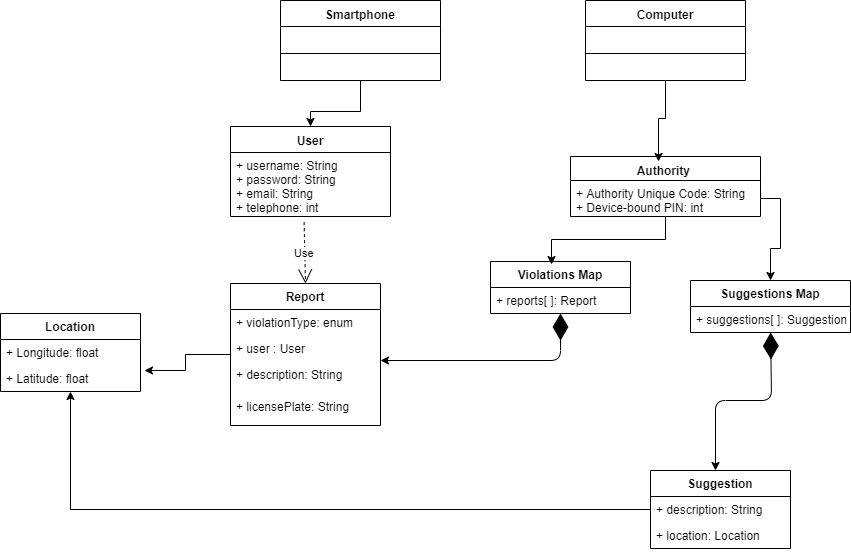
\includegraphics[width=1.0\linewidth]{assets/images/exports/user/UML.png}
						\caption{UML Class Diagram}
						\label{}
					\end{figure}
Finally, below are two UML Statechart Diagrams, one for the user and the second one for authorities
					\begin{figure}[H]
						\centering
						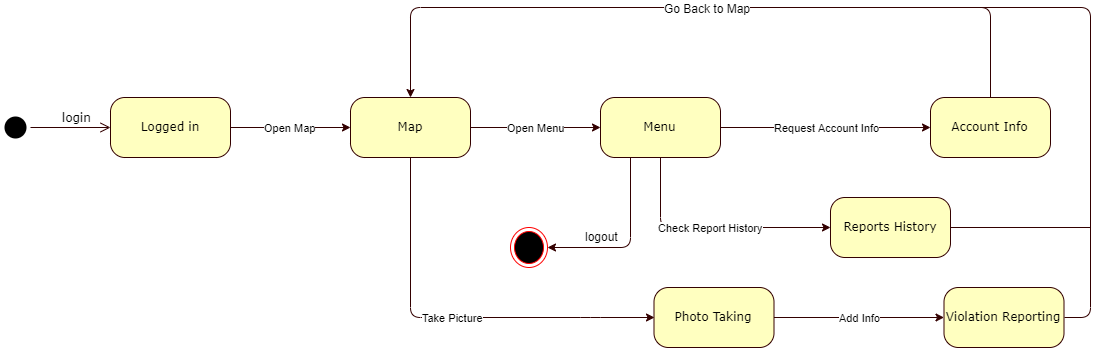
\includegraphics[width=1.0\linewidth]{assets/images/exports/user/StateChartDiagramUser.png}
						\caption{Users' Statechart Diagram}
						\label{}
					\end{figure}
					\begin{figure}[H]
						\centering
						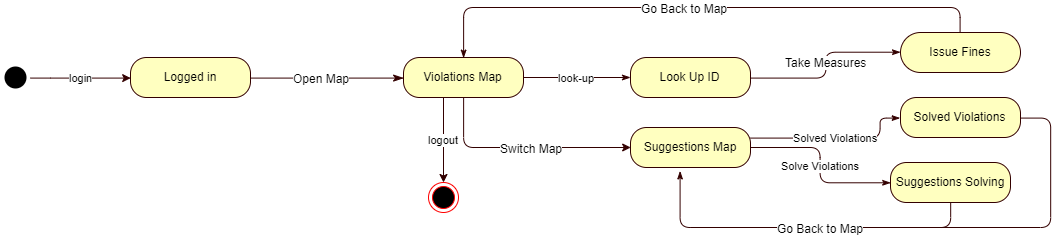
\includegraphics[width=1.0\linewidth]{assets/images/exports/authority/StateChartDiagramAuthority.png}
						\caption{UML Class Diagram}
						\label{}
					\end{figure}

\subsection{Product functions} 
According to the goals defined in the first section, we can list the most important functions the system needs to work correctly:
\begin{itemize}
\item {\texttt{Registration and Login}}: This functionality enables users to register to the system by inserting their personal data, and to login with their chosen username and password. The system must therefore store the data in it's database and retrieve it when queried.  
\item {\texttt{Violation Reporting}}: The system must provide users with an in-app photo sending functionality where users can send pictures of the vehicles' plate, select the type of violation from the dropdown menu and let their GPS track down their position.
\item {\texttt{Reports History}}: The system must allow users to access their reports history, where all those users' previous reports are stored with their data (type, location etc.)
\item {\texttt{Violations/Suggestions Map}}: The software must cross its report positions with the municipality to identify unsafe areas and highlight them on a map together with their suggestions.
\item {\texttt{Violation Solving}}: The system must enable authorities to access the map of violations and as soon as measures are taken, check them as "solved".
\end{itemize}

\newpage

\subsection{User characteristics} 
\begin{itemize}
\item {\texttt{Registered User}}: A person who registered to SafeStreets, sharing his personal data. He can login to the system by providing credentials and exploit all the services.
\item {\texttt{Authorities}}: A Law Enforcement agent who has direct access to the users' reports on their web app and can issue warnings, fines and measures.
\end{itemize}
\subsection{Assumptions, dependencies and constraints}
 \begin{itemize}
				\item {\textbf[}\textbf{D1}{\textbf]}: Users' must provide valid credentials when registering to the system
				\item {\textbf[}\textbf{D2}{\textbf]}: The license plate must be clearly visibile in the photo
				\item {\textbf[}\textbf{D3}{\textbf]}: Users' device must support the GPS technology
				\item {\textbf[}\textbf{D4}{\textbf]}: Users' device must support Mobile Applications
				\item {\textbf[}\textbf{D5}{\textbf]}: Users' device must be connected to the internet
				\item {\textbf[}\textbf{D6}{\textbf]}: Users' device must have a camera
				\item {\textbf[}\textbf{D7}{\textbf]}: Users' must always take pictures of vehicles only
				\item {\textbf[}\textbf{D8}{\textbf]}: Users' can't load photos from their device 
				\item {\textbf[}\textbf{D9}{\textbf]}: The verification e-mail/SMS will be received by the user 	
				\item {\textbf[}\textbf{D10}{\textbf]}: Authorities must have access to the internet
				\item {\textbf[}\textbf{D11}{\textbf]}: Authorities must be provided with their authority identification
				\item {\textbf[}\textbf{D12}{\textbf]}: Authorities must always check the validity of the photos taken
			\end{itemize}

\newpage

\section{SPECIFIC REQUIREMENTS}
\subsection{External Interface Requirements} 
\subsubsection{User Interfaces}
These mockups represent an idea of how the user's interface will be shown and easily accessed, spanning from the simple registration and login to the violation report function. 
\\ \\
You can also notice how SafeStreets provides the authorities' with a Web App which is separated both in functions and in design from the normal mobile app destinated to users.
					\begin{figure}[H]
						\centering
						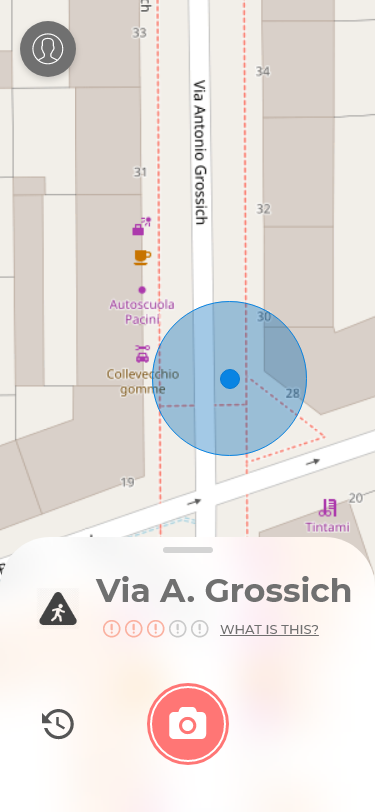
\includegraphics[width=0.4\linewidth]{assets/images/exports/user/home.png}
						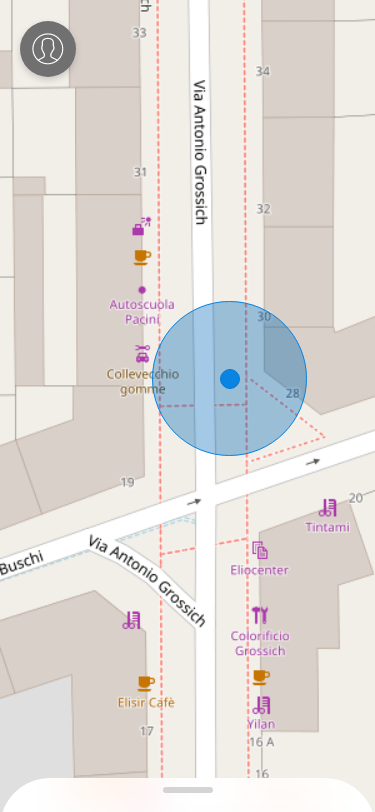
\includegraphics[width=0.4\linewidth]{assets/images/exports/user/home-no-map.png}
						\caption{The Homepage with its photo button}
						\label{}
					\end{figure}
				\begin{figure}[H]
						\centering
						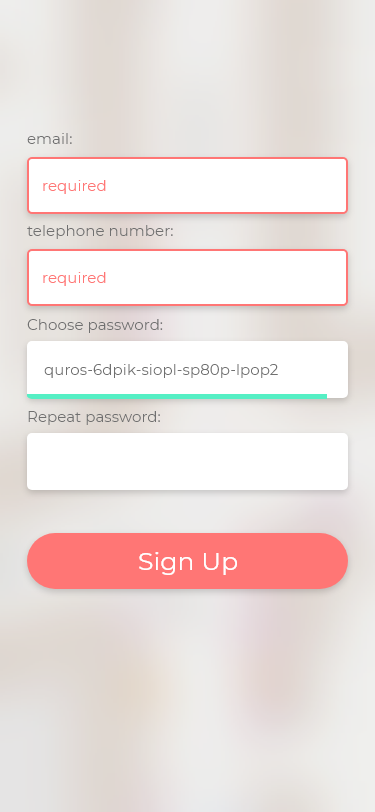
\includegraphics[width=0.3\linewidth]{assets/images/exports/user/sign-up.png}
						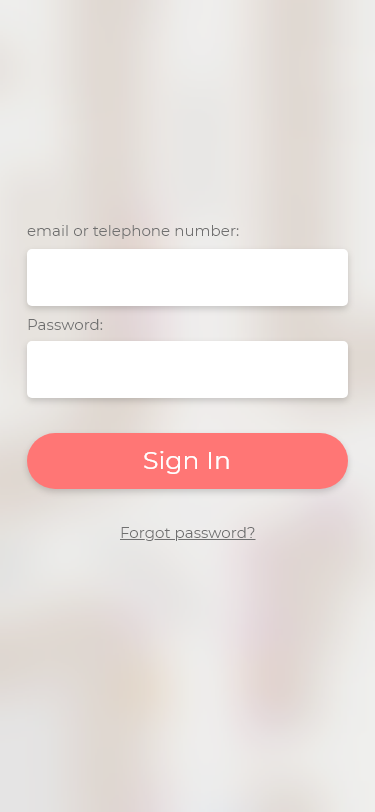
\includegraphics[width=0.3\linewidth]{assets/images/exports/user/sign-in.png}
						\caption{The registration and login pages where you input your credentials}
						\label{}
					\end{figure}
					\begin{figure}[H]
						\centering
						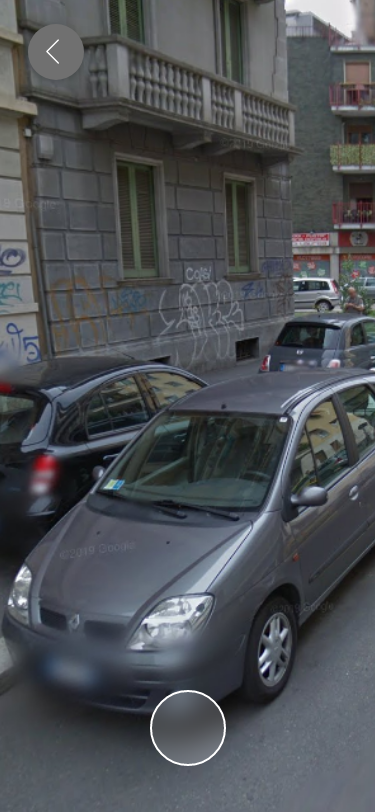
\includegraphics[width=0.3\linewidth]{assets/images/exports/user/take-photo.png}
						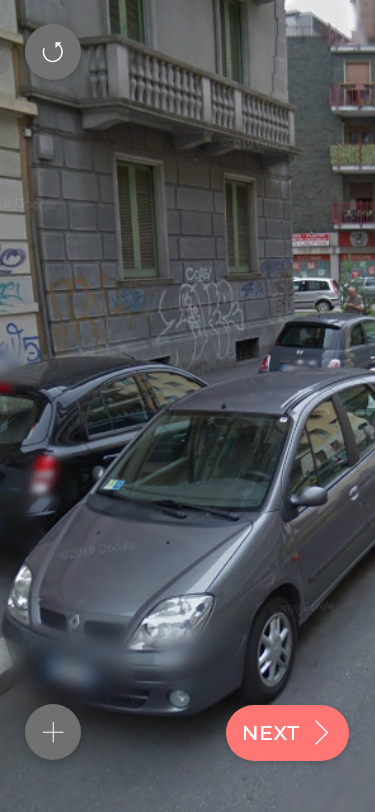
\includegraphics[width=0.3\linewidth]{assets/images/exports/user/confirm-photo.png}
						\caption{Snapshots from the photo-taking screen and the confirmation photo}
						\label{}
					\end{figure}
					\begin{figure}[H]
						\centering
						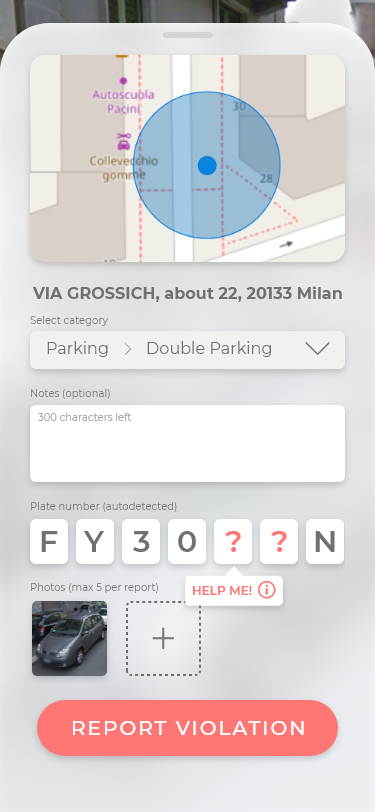
\includegraphics[width=0.3\linewidth]{assets/images/exports/user/violation-details.png}
						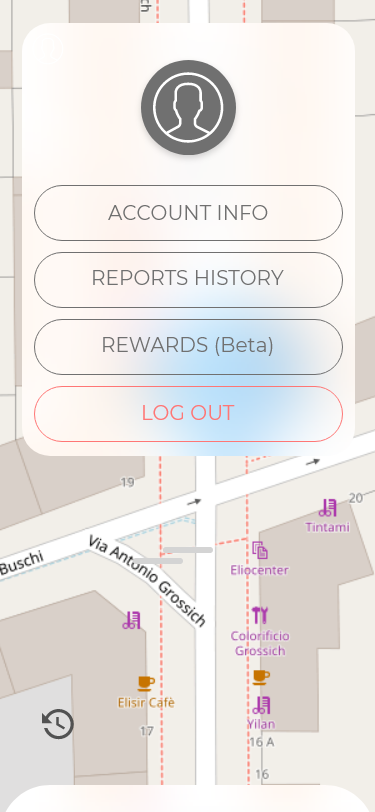
\includegraphics[width=0.3\linewidth]{assets/images/exports/user/account-info.png}
						\caption{The Violation Reporting functionality and the menu}
						\label{}
					\end{figure}
					\begin{figure}[H]
						\centering
						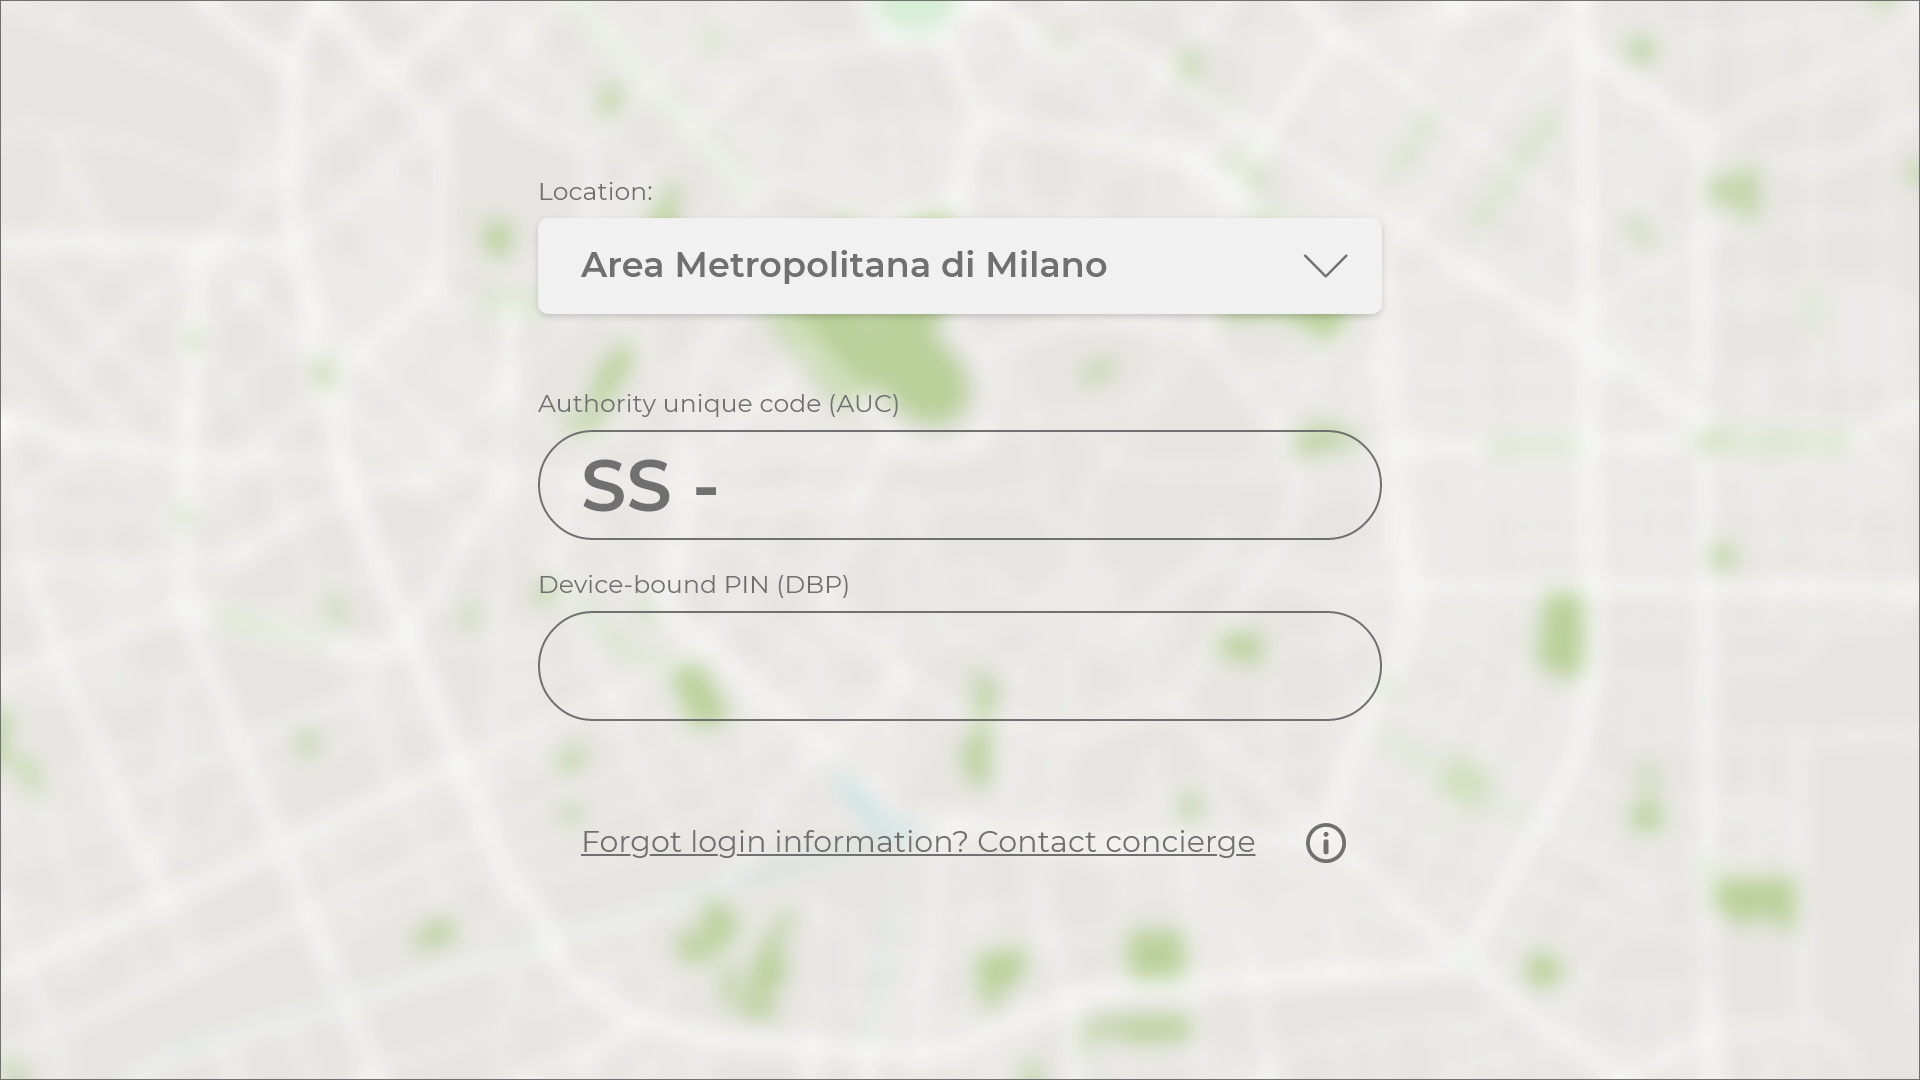
\includegraphics[width=1.0\linewidth]{assets/images/exports/authority/sign-in.png}
						\caption{The login page for authorities}
						\label{}
					\end{figure}
					\begin{figure}[H]
						\centering
						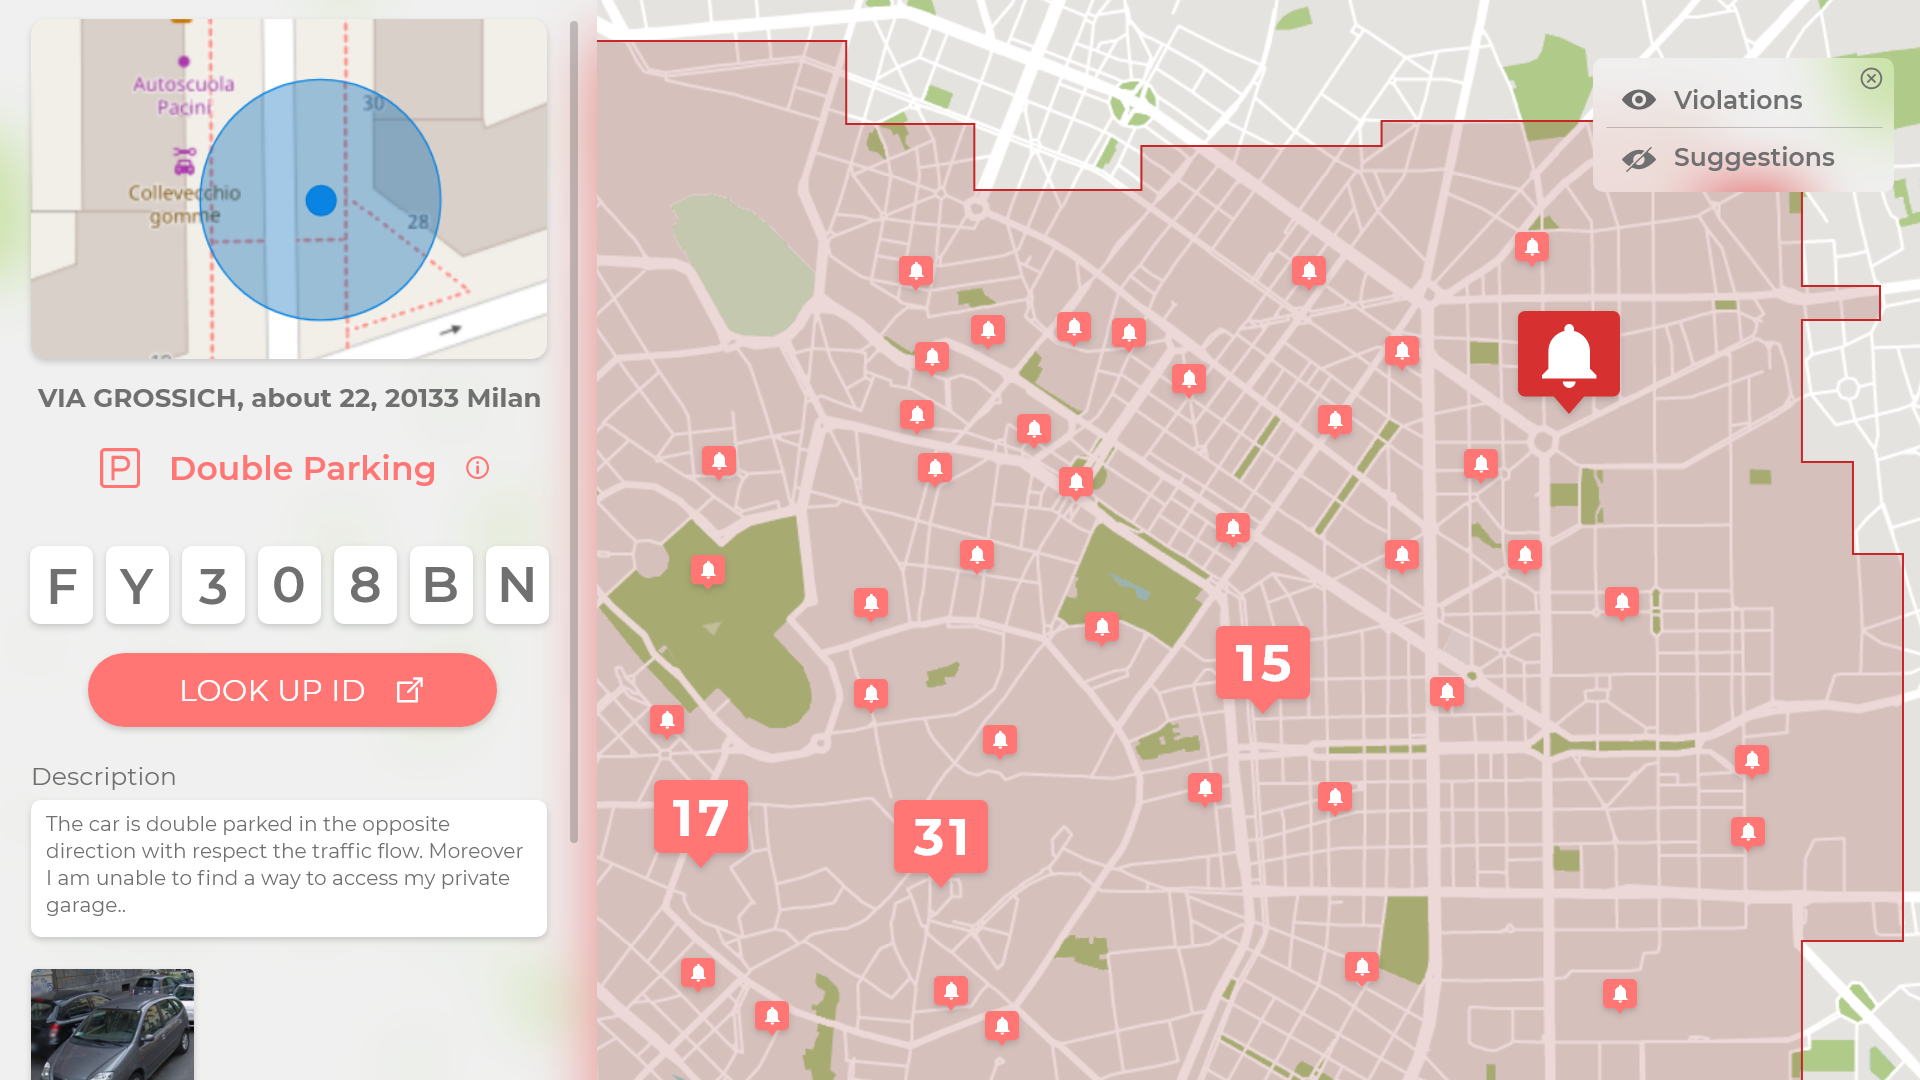
\includegraphics[width=1.0\linewidth]{assets/images/exports/authority/reports-list.png}
						\caption{The Violations Map where authorities can post suggestions or look-up license plates}
						\label{}
					\end{figure}
 					\begin{figure}[H]
						\centering
						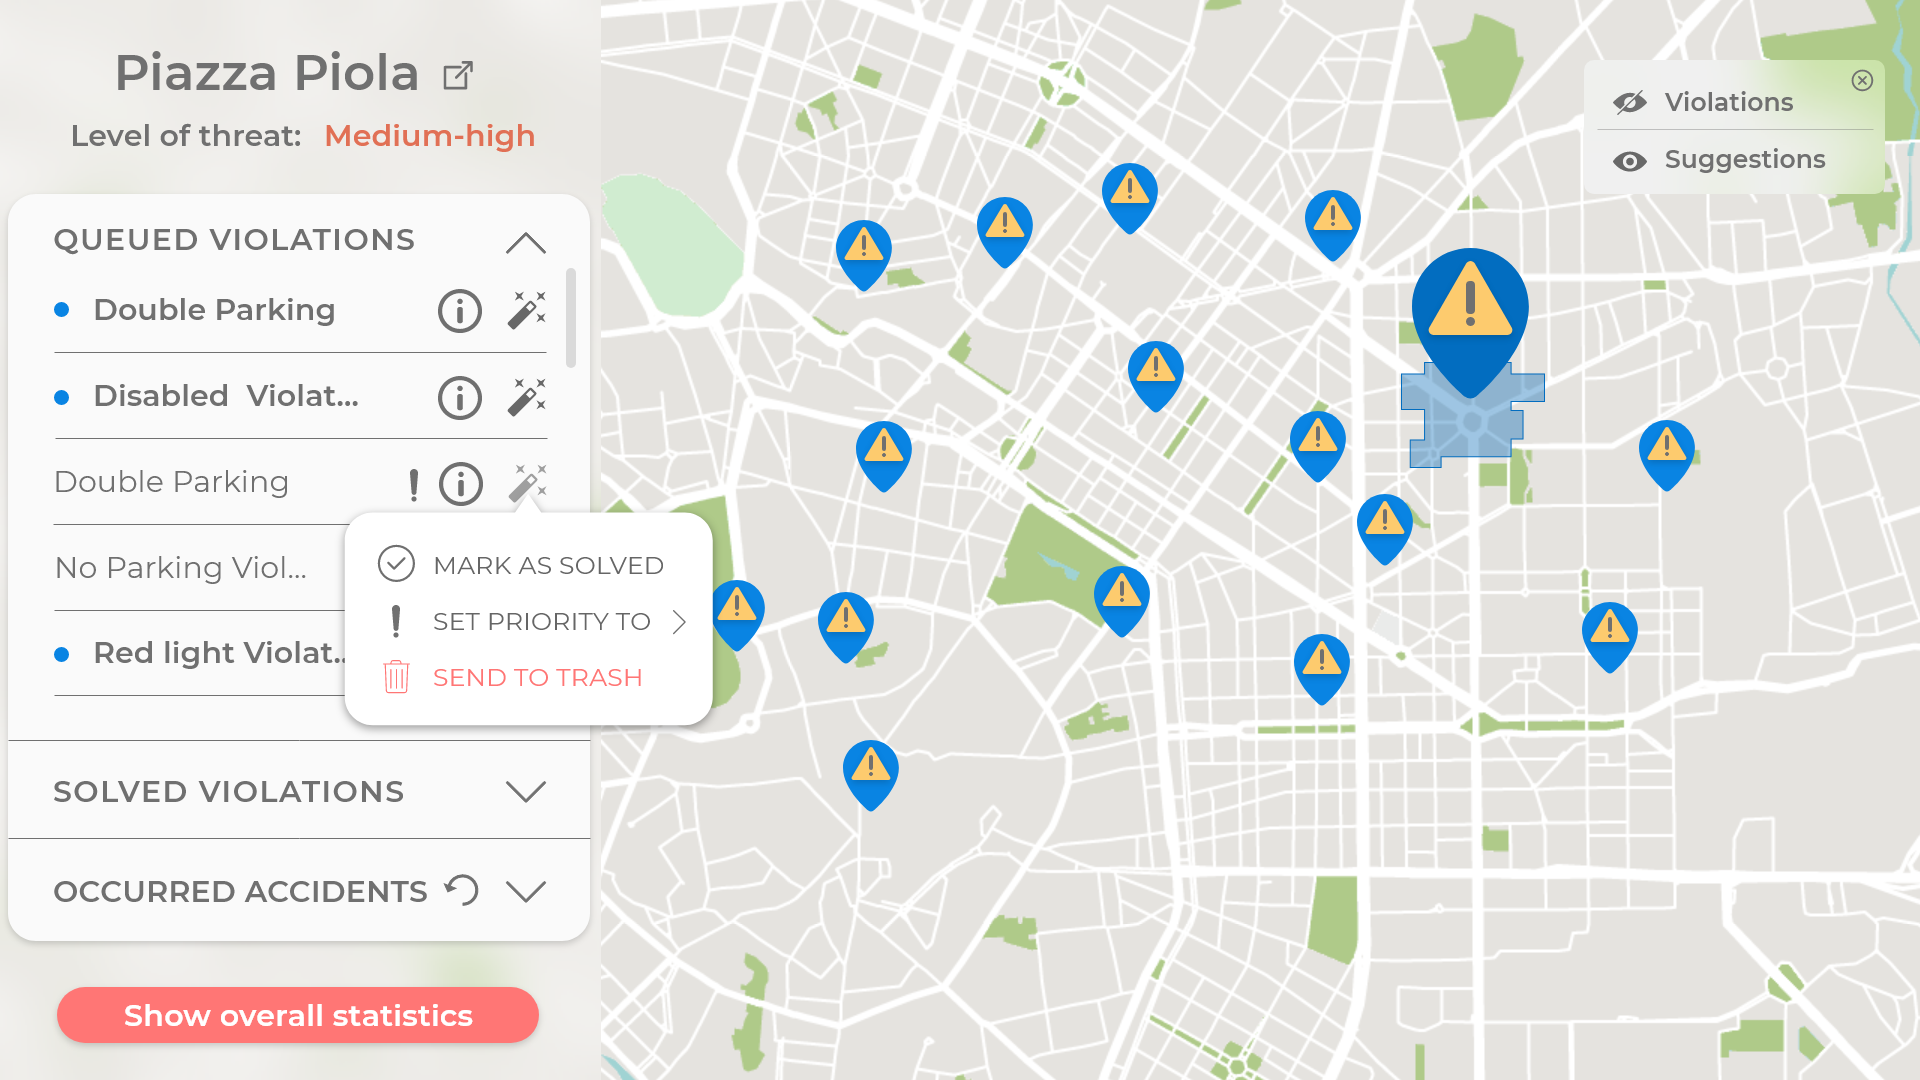
\includegraphics[width=1.0\linewidth]{assets/images/exports/authority/suggestions-list.png}
						\caption{The Suggestions Map where authorities can solve violations}
						\label{}
					\end{figure}
		\newpage
\subsubsection{Hardware Interfaces}
The application must run over the Internet, therefore all the hardware must connect to the network and there will be an hardware interface for the system, both server and client side.
		\begin{itemize}
			\item Server-side: e.g. Modem, WAN - LAN, Ethernet Cross-Cable.
			\item Client-side: e.g. Wi-Fi 802.11ac+ antenna, 3G/4G antenna.
		\end{itemize}
\subsubsection{Software Interfaces}
SafeStreets will provide an API for the user, together with the already Web Application Interface for authorities.\\
		More specifically, it will provide an API that allows users to report violations and check their reports history, and an API for authorities which enables them to check the Violations/Suggestions Map and take measures.
\subsubsection{Communication Interfaces}
Exploits all the basic network information transporting protocols, such as TCP and UDP, sockets and RMI \\
	\newpage
\subsection{Scenarios}
\subsubsection*{Scenario 1 - User Registration}
Marco decides to contribute to his cities' street security by registering to SafeStreets. He opens the app, and he inserts his personal data, such as name, surname and e-mail. He then decides a username and a password to access the app. He is now ready to report violations and secure the city.
\subsubsection*{Scenario 2 - Authority Registration}
Giovanni is a policeman who wants to register as an authority on the system. He makes a special request, sending his personal information and his authority identification to the system which checks it's validity and sends back to Davide an Authority Unique Code (AUC), which he will need to login, and a Device-bound PIN (DBP), which is bound to special devices in dotation to authorities only. He can now check the users' reports, issue fines and check the Unsafe Areas Map. 
\subsubsection*{Scenario 3 - Violation Report}
Roberto is a guy who lives in a street constantly full of double-parked cars. Tired of this situation, he decides to report them to the authorities throughout SafeStreets. He takes a picture of the car with the license plate fully visible, he lets the app track down his position and he selects a type of violation from the dropdown menu.
\subsubsection*{Scenario 4 - Suggestion Report}
Ciro is in his office watching the Unsafe Areas map of his city. In particular, he notices that there's an area in his city full of reports and violations of cars parking in the bike lane and therefore occupying it. So he decides to use the suggestion report function to hint the municipality in placing a protection barrier parallel to the edge of the bike lane in order to prevent cars from parking on them.
\newpage
\subsection{Functional Requirements}
\subsubsection*{{[}{G1}{]}: Allow users to register to the system with their personal data}
\begin{itemize}
\item {[D1]}: Users' must provide valid credentials when registering to the system
\item {[D4]}: Users' device must support Mobile Applications
\item {[D5]}: Users' device must be connected to the internet
\item {[D9]}: The verification e-mail/SMS will be received by the user 
\\\\
\item {[R1]}: The system must allow users to provide their credentials and personal data
\item {[R2]}: The system must let the user verify his account with his e-mail or by SMS
\item {[R3]}: The system must verify there are no other registered users with the same e-mail or telephone number
\item {[R4]}: In order to register successfully, the system must oblige the user to accept the data privacy policies and conditions
\end{itemize}
\subsubsection*{{[}{G2}{]}: Allow users to report traffic/parking violations}
\begin{itemize}
\item {[D2]}: The license plate must be clearly visibile in the photo
\item {[D3]}: Users' device must support the GPS technology
\item {[D5]}: Users' device must be connected to the internet
\item {[D6]}: Users' device must have a camera
\item {[D7]}: Users' must always take pictures of vehicles only
\item {[D8]}: Users' can't load photos from their device 
\\\\
\item {[R5]}: The system must give the user the possibility to take pictures
\item {[R6]}: The system must retrieve the users' position correctly
\item {[R7]}: The system must recognize the license plate 
\item {[R8]}: The system must give the user the chance to select a violation type from the dropdown menu
\item {[R9]}: The system musn't give the user the possibility to load photos from their device
\item {[R10]}: If the users' wants to, the system must let them write an optional description.
\end{itemize}
\subsubsection*{{[}{G3}{]}: Allow users to check their reports history}
\begin{itemize}
\item {[D4]}: Users' device must support Mobile Applications
\item {[D5]}: Users' device must be connected to the internet
\\\\ 
\item {[R11]}: The system must show to the user all the violations he reported in the past
\end{itemize}
\subsubsection*{{[}{G4}{]}: Allow users to check their account info}
\begin{itemize}
\item {[D4]}: Users' device must support Mobile Applications
\item {[D5]}: Users' device must be connected to the internet
\\\\
\item {[R12]}: The system must show to the user his account information and personal data when requested
\end{itemize}
\subsubsection*{{[}{G5}{]}: Allow authorities to register to the system with their personal data}
\begin{itemize}
\item {[D10]}: Authorities must have access to the internet
\item {[D11]}: Authorities must be provided with their authority identification
\\\\
\item {[R13]}: The system must allow authorities to provide their credentials and personal authority identification
\item {[R14]}: The system must verify there are no other registered authorities with the same identification
\item {[R15]}: In order to register successfully, the system must oblige the authority to accept the data privacy policies and conditions
\end{itemize}
\subsubsection*{{[}{G6}{]}: Allow authorities to access the Violations/Suggestions map}
\begin{itemize}
\item {[D10]}: Authorities must have access to the internet
\item {[D12]}: Authorities must always check the validity of the photos taken
\\\\
\item {[R16]}: The system must allow authorities to access the Violations Map and see which type of violations are being committed where
\item {[R17]}: The system must allow authorities to switch to the Suggestions Map and see which suggestions have been posted for each area
\end{itemize}
\subsubsection*{{[}{G7}{]}: Allow authorities to suggest interventions or take measures}
\begin{itemize}
\item {[D10]}: Authorities must have access to the internet
\\\\
\item {[R18]}: The system must allow authorities to suggest interventions
\item {[R19]}: The system must allow authorities to take measures such as issuing fines etc.
\end{itemize}
\subsection{Performance Requirements}
	The system must be able to handle a big quantity of reports with several images attached throughout the day. In order to improve the performance of the system, SafeStreets should rely on lightweight TCP connections.\\
	For what concerns the Violations/Suggestions Map, the map scrolling must be fluid and responsive, the violation alerts clear and the login process for both users and authorities must be fast and reliable
\subsection{Design Constraints}
\subsubsection{Standards compliance}
Since the system processes sensitive data, the software complies to the General Data Protection Regulation (GDPR), a european regulation law on privacy policies and data protection for all the individuals living within the European Union (EU)
\subsubsection{Hardware limitations}
	\begin{itemize}
			\item \texttt{Mobile App}: 
				\begin{itemize}
					\item Smartphones: iOS/Android, Internet Connection, GPS, camera.
				\end{itemize}
			\item \texttt{Web App}: modern web browser (e.g. Google Chrome / Safari), specifically intended for authorities only, enabled by the above said communication protocols and APIs.
		\end{itemize}
%\subsubsection{Any other constraint}
\subsection{Software System Attributes} 
\subsubsection{Reliability}
The system must be active 24/7
\subsubsection{Availability}
Whenever requested (a user wants to report a violation immediately or a user wants to register), the system must respond correctly and rapidly to the queries
\subsubsection{Security}
Since personal information is stored, the system guarantees not to divulgate them to unauthorized third parties, with respect to the GDPR
\subsubsection{Maintainability}
Enforced by the usage of specific design patterns and the provided hardware/software requirements, the software must be easy to fix and modifiy (or maintain) in the future
\subsubsection{Portability}
The software is generally projected for every type of mobile device, such as tablets and smartphones, and every type of OS, such as iOS or Android. Specifically for authorities, the Web App is compatible with every known browser  
\section{FORMAL ANALYSIS USING ALLOY: This section should include a brief presentation of the 
main objectives driving the formal modeling activity, as well as a description of the model 
itself, what can be proved with it, and why what is proved is important given the problem at 
hand. To show  the soundness and correctness of the model,  this section can show some
worlds obtained by running it, and/or the results of the checks performed on meaningful 
assertions}
\section{EFFORT SPENT}
\begin{itemize}
		\item Giancarlo Danese
		\begin{center}
			\begin{tabular}{| c | c | c |}
				\hline
				Day & Subject & Hours \\ \hline
				18/10/2019 & Purpose, Scope & 2 \\
				23/10/2019 & Domain Assumptions, User Characteristics & 1.5 \\
				28/10/2019 & Definitions, Acronyms, Product Functions & 1 \\
				30/10/2019 & Scenarios, Domains & 2 \\
				\hline
			\end{tabular}
		\end{center}

		\item Davide Savoldelli
		\begin{center}
			\begin{tabular}{| c | c | c |}
				\hline
				Day & Subject & Hours \\ \hline
				18/10/2019 & Goals, Product Functions & 1 \\
				23/10/2019 & Document Structure & 2 \\
				28/10/2019 & User Interfaces, Mock-ups & 3 \\
				30/10/2019 & Goals, Requirements & 1 \\
				\hline
			\end{tabular}
		\end{center}
	\end{itemize}
\section{REFERENCES}


\end {document}